\documentclass[11pt]{article}
\usepackage{fullpage,ifthen,enumerate,algo,url}
%\usepackage[pdftex]{graphicx}
\usepackage{graphicx}

\begin{document}
%
% Headings
%
\begin{center}
UNIVERSITY OF WATERLOO\\
Cheriton School of Computer Science\\[\baselineskip]
{\bf CS240\hfill Data Structures and Data Management \hfill
Winter 2013}\\[\baselineskip]
{\sc \large ASSIGNMENT 5}\\
(Due: Monday, April 1, 2013, 9:30am)\\[2\baselineskip]
\end{center}
%
% Main body
%

%\maketitle
\noindent


Please read \url{http://www.student.cs.uwaterloo.ca/~cs240/w13/guidelines.pdf} for guidelines on submission. 
All problems except for 3 are written problems; submit all of your solutions as a PDF file named {\tt a05w.pdf}, or for individual questions submit files named {\tt a05q1w.pdf}, ... , {\tt a05q10w.pdf}. 
Implement the solution for Problem 3 in C++ and submit files named {\tt a5q3.\{cpp,h\}}. 
Make sure the code you submit runs in the student environment.
\noindent
\begin{enumerate}

\item The worst case of interpolation search results in $\Theta(n)$ search time. 
Let $i$ be the interpolated index where the next comparison in the search will be made (formula taken from them lecture notes): 
\[ i = \ell+\left\lfloor\frac{k-A[\ell]}{A[r]-A[\ell]}(r-\ell)\right\rfloor \]

This splits the array into two parts, a smaller ``good side'' and a larger ``bad side''. 
A recursion on the ``bad side'' is called an \emph{interpolation failure}.

Assume we keep track of the interpolation failures in a counter called {\tt numFailures}. 
We wish to devise a new interpolated index formula based on {\tt numFailures} that adjusts the value $i$ to make the two parts more balanced, hopefully avoiding some future interpolation failures.

\begin{enumerate}
\item {[5 marks]}  Give pseudocode for a modified interpolation search in which the two parts are made more balanced by reducing the size of the larger side by up to {\tt numFailures}.
Make sure to handle boundary cases.
\item {[5 marks]}  Give the worst case search time for this procedure.
\item {[5 marks]}  Give pseudocode for a modified interpolation search in which the two parts are made more balanced by reducing the size of the larger side by up to the value of $2^{\mbox{\small\it numFailures}}$.
Make sure to handle the boundary cases.
\item {[5 marks]} Give the worst case search time for this procedure.
\end{enumerate}

{\bf Example.}
Consider this output from an interpolation search:
\begin{verbatim}
k = 66, A = { 6, 35, 42, 58, 59, 67, 68, 82, 85, 96 }
Iteration 1: l = 0, r = 9, i = 6
Iteration 2: l = 0, r = 5, i = 4
k = 66 not found
\end{verbatim}
The first iteration of the search compares the key to {\tt A[6] = 68} and then recurses/iterates on the left since {\tt k < A[6]}.
Since there are 3 indices on the right of {\tt A[6]} and 6 indices on the left, the right is the good side and the left is the bad side, so recursing on the left in this case is an interpolation failure.

\item {[10 marks]}  
Galloping is sometimes called a one-sided binary search.
Describe a one-sided interpolation search in which instead of searching at locations 1, 2, 4, 8,\ldots we interpolate (more precisely, extrapolate) the next location to be probed on the basis of the locations we have already seen.
More specifically, given array A and search key k, find a formula for $i_n$, the index of the next probe in the search (assume that $i_{n-1}, i_{n-2}, \ldots$ were also generated by the formula).
Hint: modify the interpolation search formula from the lecture notes.

\item {[10 marks]}  
Download and then resubmit {\tt a5q3.\{cpp,h\}} after implementing {\tt SkipList::SkipList( const std::vector<int>\& )}. 
In particular, given $n$ unique, sorted input values, the function must build a {\bf deterministic} perfectly balanced skip list with $\lg n$ levels in which exactly every other element from the previous level is promoted to the level above.

You may modify or add to the code as you see fit, but do not change the prototypes of the given functions.

{\bf Examples.}
\begin{verbatim}
{ 0 } --> -inf 0 inf

{ 0, 1 } --> -inf---1-inf
             -inf-0-1-inf

{ 0, 1, 2 } --> -inf---1---inf
                -inf-0-1-2-inf

{ 0, 1, 2, 3 } --> -inf-------3-inf
                   -inf---1---3-inf
                   -inf-0-1-2-3-inf
\end{verbatim}

\item 	{[5 marks]}
One of the applications of quad trees is compression of pictures. The picture is recursively divided in quadrants until the entire quadrant is of the same colour. Using this rule, draw the quadtree of the following picture.

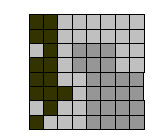
\includegraphics[width=50mm]{image.png} 

\item {[5 marks]} Draw the kd-tree on the points

(1,12) (3,11) (5,10) (7,9) (9,5) (11,6) (13,7) (15,8) 
(2,4) (4,3) (6,2) (8,1) (10,15) (12,14) (14,13) 

\item {[5 marks]} Draw the balanced range tree on the same set of points, i.e.

(1,12) (3,11) (5,10) (7,9) (9,5) (11,6) (13,7) (15,8)
(2,4) (4,3) (6,2) (8,1) (10,15) (12,14) (14,13)


\item {[5 marks]} Senator Raul Payn likes simplistic solutions to complicated problems. He believes
that range trees are a waste of pointers and government money so he chooses to eliminate
the y-coordinate trees and make do with with a balanced BST on the x-coordinates first.
Construct an example of a set of $n$ points and a query rectangle such that the 
(1) the answer is empty and (2) the total number of points examined to answer the
query using an x-coordinate tree is $n$.


\item	{[8 marks]} Consider the Boyer-Moore pattern matching method using only the bad character heuristic as seen in class. Let the alphabet be \verb+{e,f,g,l}+.
    
\begin{enumerate}
\item 	First, compute the shift function for each character of the alphabet over the pattern {\tt gell}
\item	In what follows we show the first few steps of the algorithm, complete the remaining steps to search the entire text. Underline the characters that are compared in each alignment before each shift.

\begin{verbatim}
feelfleeflegellfellgellglee
gell
 gell
\end{verbatim}
\end{enumerate}

\item {[20 marks]}

\begin{enumerate}
\item
	 Show in a diagram the suffix trie for \verb+kneel knell knead keel+.
\item
	 Show in a diagram the suffix trie for \verb+00111000111001$+.
\item
	 Show in a diagram the suffix tree for \verb+kneel keel knell knead+.
\item
	 Show in a diagram the suffix tree for  \verb+00111000111001$+.
\item
 Prove that the suffix trie of a string has $m^2$ nodes when the string is of the form \verb+00...0011...1100...0011...11+ where $m$ is the number of consecutive 0s and 1s.
\end{enumerate}

\item After writing his memoirs, Foghorn Leghorn has decided to compressed them using
      Lempel-Ziv compression with six bit codes.  The code table is initialized only with the codes (a,000000), (b,000001), \ldots, (z,011001) (space, 011010), (', 011011), (, ,011011).  Compress the opening sentence "that's a joke, that's a joke, son, that's a joke".
      
      Given the amount of repetition in the sentence above, comment on the quality of
      compression of LZW in this instance. 
      
      Using the table above decompress 
      
      {\tt 00000000011110010001001000001011011011010010011010000101001110001110001011}
 
\end{enumerate}


\end{document}
